\title{Simulation using Hamiltonian Monte Carlo}
\author{
        Ho Chung Leon  Law \\
            \and
        Nathan Cunningham\\
}
\date{\today}

\documentclass[11pt]{article}
\usepackage{amsmath}
\usepackage{algorithm}
\usepackage{algpseudocode}
\usepackage{graphicx}
\usepackage{amssymb}
\usepackage{hyperref}
\usepackage[a4paper,bindingoffset=0.2in,%
            left=1in,right=1in,top=1in,bottom=1in,%
            footskip=.25in]{geometry}
\begin{document}
\maketitle

\begin{abstract}
In this report we aim to examine the properties of Hamiltonian Monte Carlo, implement it in the R coding language, and compare its effectiveness to another method of monte carlo simulation. \ldots
\end{abstract}
\newpage
\section{Introduction}
Popular methods to simulate from a density of interest include Random Walk Metropolis-Hastings and Gibbs Sampling, however, these may have slow mixing properties, especially in a high-dimensional setting. Hamiltonian Monte Carlo (HMC) makes use of first-order gradient information of the target density and Hamiltonian dynamics, allowing us to coherently explore the state space. This is done through the introduction of auxiliary momentum variables, which allows the use of Hamiltonian dynamics to construct an ergodic markov chain, whose stationary distribution is our density of interest. 
\\
\\
In this report, we will first give a quick overview and intuition of the HMC algorithm, which is primarily based on Neal\cite{neal} and Duane et al\cite{duane}. We will then go on to implement the algorithm in R and compare results to those obtained from from different samplers, such as random walk Metropolis Hastings, HMC and No-U-Turn Sampler (NUTS). We will also illustrate these methods on multivariate Gaussian mixture models, whose densities represent the 26 letters of the alphabets (upper and lower Case), where the mixtures were found by using the EM-algorithm on an image data set of alphabets.
\section{Hamiltonian Monte Carlo}
\subsection{Hamiltonian dynamics}
We will first describe Hamiltonian dynamics, before stating how we will utilise them in the next section. Hamiltonian dynamics is the system described by a pair of differential equations with coordinates $(q,p)$, for $i=1 \dots d$
\begin{equation}
\frac{dq_{i}}{dt} = \frac{\delta H}{\delta p_{i}}
\end{equation}
\begin{equation}
\frac{dp_{i}}{dt} = \frac{-\delta H}{\delta q_{i}}
\end{equation}
where $H$ is called the Hamiltonian and is a function of time and $(q,p)$. This system in fact arises from Newtonian Mechanics, and has a natural interpretation in physics and in nature. If we think of $(q(t),p(t))$ as 2 dimensional position and momentum  vectors at time t respectively and the Hamiltonian as the simply the sum of the kinetic (function of momentum) and potential energy (function of its position), we can just think of the equations as describing the evolution of a friction less particle over time. We will now set up our notation and the introduce the idea of an energy function.
\subsection{Target Density and Energy Function}
We first define our target density to be of the form (without normalising constant):
\begin{equation}
P(q)= \pi(q)L(q|D) \quad \quad q \in \mathbb{R}^{d}
\end{equation}
where $\pi(q)$ is the prior density and $L(q|D)$ is the likelihood given data $D$. 
We also define $q$ to be the `position' vector in $d$ dimensions. Now, from statistical mechanics, given some energy function $E(x)$ in some system, we can express its canonical distribution as:
\begin{equation}
\label{energy}
Pr(x) = \frac{1}{Z}exp(-E(x)/T)
\end{equation}
where $T$ is the temperature of the system (which we assume to be 1) and $Z$ is a normalising constant. By considering this, we define the energy of our target density as:
\begin{equation}
U(q) = -log[\pi(q)L(q|D)]
\end{equation}
We now introduce an auxiliary variable $p$ (`momentum' in $d$ dimensions), which we define to have energy function $K(p)$, which using equation (\ref{energy}) has in turn a density function $Q(p)$ say. We then define the joint density of $(p,q)$ as 
\begin{equation}
P(q,p) = \frac{1}{Z}exp(-U(q)/T)exp(-K(p)/T) = \frac{1}{Z}exp(-H(q,p)/T)
\end{equation}
where $H(q,p) = U(q) + K(p)$ now can be seen as the energy function for the joint state $(q,p)$ distribution. The construction of independence between $q$ and $p$ may seem meaningless at first, but this introduction enables us to use Hamiltonian Dynamics, which has some important properties that is crucial to our construction of the Markov chain.
%allows easy extraction of samples from $P(q)$ and we remark that the introduction of $p$ 

\subsection{Properties of Hamiltonian dynamics}
We will now briefly state several important properties of the Hamiltonian, which are crucial to the HMC algorithm, before stating the relationship between the dynamics and our $P(q,p)$ density. Firstly, the the dynamics keeps the Hamiltonian invariant, i.e. the Hamiltonian is constant, this means the mapping $T_s: (q(t),p(t)) \rightarrow (q(t+s),p(t+s))$, where the arrow represents the evolution of the system is independent of time. This brings us to the second property, which says that the mapping $T_s$ is reversible, in the sense that it is a one to one mapping. This reversible property is important to show the Markov chain constructed in Algorithm () satisfies detail balance and hence leave the desired distribution invariant. The third important property is that Hamiltonian dynamics preserves volume in the $(q,p)$ space, in the sense that the image of $T_s$ to some region R has the same volume as region R. This property means that there is no need to account for any change in volume in the acceptance probability of Metropolis Hastings, where for general dynamics will be infeasible to compute. To understand these exact properties and how they are used in the proof of this algorithm, see .
\subsection{Hamiltonian Dynamics and Hamiltonian Monte Carlo}
Because of these nice properties of the Hamiltonian dynamics, we may like to construct a Hamiltonian and Markov chain that make use of these properties. This is exactly our $H(q,p)$ we defined early in equation (), where we have introduced an `momentum' variable p. Looking at the form of the Hamiltonian, we can in fact attach our previous physical interpretation of `potential' ($U(q)$) and 'kinetic' energy ($U(p)$) to it. 
\\
\\
As an illustration, let $P(q)$ be an univariate gaussian, which means $U(q)=\frac{q^2}{2}$. So now imagine we put a particle on the energy function of this gaussian and give it some momentum in some direction, then Hamiltonian dynamics is then exactly describing the transfer of energy between $U(q)$ and $P(q)$, as the Hamiltonian is conservative. So given sufficiently energy, the particle will in fact `travel' a sufficiently `large' amount of the state space of the position vector $q$ in some time period. HMC basically make use of this by constructing a new position state from the previous position state by stoping the dynamics after initialising from previous position state and some random momentum. It is important to note here, unlike proposals in Random Walk Metropolis Hastings, due to the properties of the Hamiltonian, the acceptance probability of this new state is always 1. 
\\
\\
This allows for coherent exploration of the state space, and in fact this exploration can be thought of as  travelling along the contours of the $-log( P(q,p)$ or equivalently the Hamiltonian energy function $H(q,p)$ due to the conservation of the Hamiltonian dynamics and the 'jump' between the contours of the energy levels is done by sampling momentum with respect to the corresponding density function of $K(p)$ This replacement of $p$ can change the probability density of $(q,p)$ by a lot amount, hence also for $U(q)$, allowing exploration.
\\
\\
We have yet to specify the energy function $K(p)$, but in theory most positive functions can be chosen. A common choice is to use the energy function from a multivariate gaussian with mean bold 0 and diagonal covariance matrix $M$.
\begin{equation}
K(p) = \sum_{i=1}^{d} \frac{p_{i}^{2}}{2m_{i}}
\end{equation}
Some reasons why this is chosen is because at every step of the Markov chain, the momentum is resampled from the density function with respect to $K(p)$ and a gaussian can be easily simulated. Also, it is also only intuitive to choose a symmetric density with an infinite support to encourage mixing of the chain, furthermore this has a very nice interpretable physical meaning, being exactly the kinetic energy form we observe in nature. 
\subsection{The Leapfrog}
In general, a solution to the Hamiltonian dynamics given an arbitrary Hamiltonian of the form $H(q,p) = U(q) + K(p)$ cannot be computed analytically. Hence we discretise the time in equation () and () with some small step size $\epsilon$ and approximate the solution to the equations using the leapfrog method:
First advance the momentum by one half-step:
\begin{equation}
p_{i}(t+\epsilon/2) = p_{i}(t) - (\epsilon/2)\frac{\delta U}{\delta q_{i}}(q(t))
\end{equation}
then advance the position by a full-step using the updated momentum:
\begin{equation}
q_{i}(t+\epsilon) = q_{i}(t) - (\epsilon)\frac{p_{i}(t+\epsilon/2)}{m_{i}}
\end{equation}
And finally advance the momentum one half-step using the updated position:
\begin{equation}
p_{i}(t+\epsilon) = p_{i}(t+\epsilon/2) - (\epsilon/2)\frac{\delta U}{\delta q_{i}}(q(t+\epsilon))
\end{equation}
Iterate over this process $L$ (Leaps) times to travel a time of $L\epsilon$.
Note this method in fact preserves volume exactly, as each step is just a shear transformation, and furthermore it is also reversible, by simply negating p and reapplying the steps. For more details on the local and global error and comparison to the Euler's Method, see >>.
\\
\\
Although the volume is conserved exactly, the value of Hamiltonian is not conserved exactly, due to the approximate error introduced by discretising. However, we will see later that this can easily be fixed using a Metropolis Hasting step. Very oftenly, there exists a critical step size, where above this value, the error of the Hamiltonian can grow without bound and below this value, the error tends to stay bounded regardless of size of L. Hence, it is important to observe the change in the Hamiltonian or the acceptance rate of the process in order to tune the size of $\epsilon$ and $L$. It is important to note that we must be able to compute the partial derivatives of the log of the density function we are interested in, and some automatic ways to do this has been proposed by: ....
%It is important to note that the particle will tend to travel in some direction, before making a u turn to come back, 

% is fact just a reformulation of Newtonian Mchanics (Newton's Laws). If we now think of 
%The Hamiltonian equations model the evolution of a particle in a frictionless system over time, $t$, given its momentum, $p$, and position, $q$. The Hamilton equation consists of the potential energy of the particle, $U(q)$, and the kinetic energy, $K(p)$, and in Hamiltonian Monte Carlo is usually written as


%Thus, we can convert our distribution $P(x)$ to a canonical distribution by setting the energy function, $E(x)$ to $-logP(x)-logZ$
\pagebreak
\subsection{The Hamiltonian Monte Carlo Algorithm}
We will now present the HMC algorithm and give some intuition behind the steps. An R package for implementation of this algorithm can be found in ... 

\begin{algorithm}
\caption{Hamiltonian Monte Carlo}\label{euclid}
\begin{algorithmic}[1] 
\State Select an initial $q$ 

\State $p\sim \mathcal{N}(0,\Sigma)$
\State Given $(q,p)$, simulate Hamiltonian dynamics using the leapfrog for $L$ steps with $\epsilon$ to find $(q^{*},p^{*})$ 
\State Negate $p^{*}$ to ensure reversibility 
\State Accept $(q^{*}, p^{*})$ as the next step in the Markov chain with probability M given below, otherwise accept $(q,p)$ as next state.
\State Return to step 2 with new state for next simulation.
\end{algorithmic}
\end{algorithm}
\noindent There are 2 main steps to the algorithm, the sampling of the momentum and the Metropolis Hastings update with Leapfrog proposal. All these steps leave the joint distribution of (q,p) invariant, and hence their combination also leave the distribution of interest invariant. In the first step (2.), new momentum are simulated from the multivariate gaussian distribution, where commonly $\Sigma$ is just the identity matrix. Due to the independence of $q$ and $p$ using our construction, the marginal density of $p$ is exactly the conditional distribution given $q$, this is in fact just basically a gibbs update, clearly this step leaves the joint distribution invariant. 
\\
\\
In the second step (3.-6.), we propose a new state $(q^{*}, p^{*})$ by simulating Hamiltonian dynamics using Leapfrog with L steps and $\epsilon$ step size. The negation of momentum in 4. ensures reversibility, although in practice this negation needs not be done as $K(p)=K(-p)$ and momentum will resampled in the next iteration. If we simulated the Hamiltonian dynamics perfectly, then we would always except the new state, as we are travelling on the contours on the (q,p) energy/density space, where the Hamiltonian is constant. However, due to approximation error, the Hamiltonian will not be conserved exactly, hence we will use Metropolis Hastings to correct for this, where the new state $(q,p)$ is accepted as the next state of the Markov chain with probability
\begin{equation}
M=min\{1,exp(-H(q^{*},p^{*})+H(q,p))\} = min\{1, exp(-U(q^{*}+U(q)-K(p^{*}+K(p))\}
\end{equation}
Note that this is just the normal Metropolis Hastings step on $(q,p)$ written in terms of the energy form. This means that a large difference in approximation error of the Hamiltonian  will in turns give a large chance of rejection, hence we can see that some tuning will be necessary to encourage of mixing of the chain. The properties of Hamiltonian dynamics means that detail balance will hold and hence leave the canonical distribution of the constructed Markov Chain invariant. For more information, refer to for informal simple proof and .. more formally. 

\subsection{Ergodicity and the choice of $L$ and $\epsilon$}
The HMC method is sensitive to the user-tuned parameters $L$ and $\epsilon$, and in fact if the solution to the equations () and () are periodic, and if $L\epsilon$ is close to this period, then trajectories from the Leapfrog will return proposals that are close to the original $q$, and hence the HMC will not give an ergodic Markov Chain. One way of solving this is to randomly choose $L$ and $\epsilon$ from some small interval routinely. Choosing $L$ and $\epsilon$ is also a major issue in HMC, for a small value of $L$, the algorithm devolves to random walk behaviour, as the position of the particle will be very dependent on the initial momentum. As going back to the previous example, where $P(q)$ is an univariate gaussian, given some position on the energy function, for a small interval of time, the particle will basically move according to the direction of the momentum and also unlikely to move far from the starting position. This is exactly like  a random walk behaviour, and also the samples are likely to be highly correlated. For L too large, it is computationally wasteful as the particle might have a performed a 'U turn' and extra work is being done to propose a $q^{*}$ that is close to our original $q$. The value of epsilon affects our the error in the Hamiltonian and could lead to a high rejection rate, if one is not careful, however too small epsilon means extra leaps will be needed to explore further.
The choice of $L$, $\epsilon$ and even $\Sigma$ takes experiences, requiring preliminary runs with different values of $L$ and $\epsilon$. But a lot of work has been done since to attempt to automate this tuning of parameters, with one important example being the No U-turn sampler (NUTS).
\subsection{No U-turn sampler (NUTS)}
The No U-turn sampler\cite{NUTS} is an implementation of an algorithm based on Hamiltonian Monte Carlo which aims to avoid the need for the user to manually specify $L$ and $\epsilon$. To find the number $L$ of leap frog steps, it uses a criterion based on half the squared distance between initial position $q$ and $q^{*}$:  
\begin{equation}
\frac{d}{dt}\frac{(q^{*}-q) \cdot(q^{*}-q) }{2}=(q^{*}-q)\frac{d}{dt}(q^{*}-q)=(q^{*}-q)\cdot p^{*}
\end{equation}
This suggests that an algorithm that runs leap frog steps until the dot product between the current momentum and $q^{*}-q$ becomes less than 0 would simulate system's dynamics until a 'U turn' occur and it starts to move back to $p$, meaning that the computation would not be too wasted or $L$ number of leaps will not be too small. However, this does not guarantee time reversibility, but NUTS uses a recursive algorithm involving trees and repeated doubling to overcome this issue. NUTS also adapts the step size $\epsilon$ on the fly based on primal-dual averaging. For more information, please refer to ...  
\section{Comparisons between HMC, MH and NUTS}
\subsection{Bivariate Gaussian simulation}
We begin by illustrate the HMC method on a bivariate gaussian with mean $(0,0)$ and standard deviations of 1 and correlation of $0.95$. For HMC, a value of $\epsilon$ of 0.20 and L=25 was chosen by looking at auto-correlation and trace plots, such that the `particle' was able to travel to a sufficiently distant point, independent of the previous point. If we examine the dynamics of the each step of the leap-frog from the starting position at say q=(-2,-2), we should see that most of the dynamics will be travelling in one direction, which is consistent with our interpretation of equation () and () in section (). In figure 1, we can see that the samples from the HMC travels a significantly large part of the state space relatively independent of the last state, with a rejection rate of 0 in this case, as the step size is relatively low. This is unlike in a random walk Metropolis Hastings (proposal of $U[-0.25,0.25]$ around current state) where even after a thinning of 25 samples, it still exhibits a highly auto-correlated behaviour and the rejection rate is at 0.4. However, the computational efficiency of both samplers on large samples has yet to tested, since proper comparisons on R is difficult.
\begin{figure}[H]
\center
  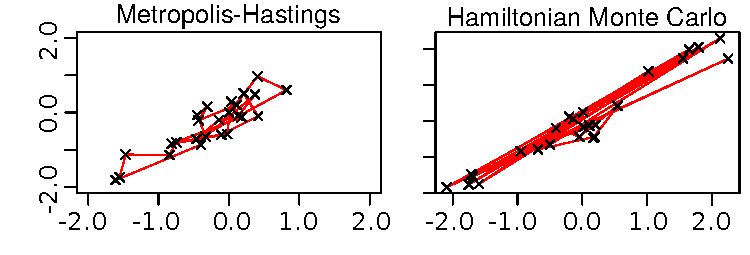
\includegraphics[width=5in]{images/MHvsHM_explore.pdf}
\caption{The trajectory of a bivariate Gaussian distribution simulated with zero-mean and marginal $\sigma$ of 1, and correlation of 0.95.}
\end{figure}
\subsection{High-dimensionality}
We will now illustrate the behaviour of random-walk Metropolis, HMC and NUTS on a 150 dimensional independent multivariate gaussian with means of 0 and increasing standard deviation of approximately 0.0065 step from 0.02 to 1. For the HMC, it was tune to have $\epsilon = 0.014$ and $L=100$, from examination of the rejection rates and diagnostic plots and also understanding that the step size is limited by the small standard deviation. Since such a small step size was chosen, it was necessary to choose a sufficiently large leap size in order to move sufficiently in the direction of large standard deviation. To avoid any possible problem with periodicity, the $\epsilon$ was randomised from an uniform of 0.014 (plus minus) 20 \%. Random walk Metropolis was also used with proposals generated from (0.02,0.03) with a thinning of 100 samples to roughly compare the computational time. The rejection rate was 0.5 for the Metropolis Hasting and 0.05 for the HMC algorithm. 
\begin{figure}[H]
\center
  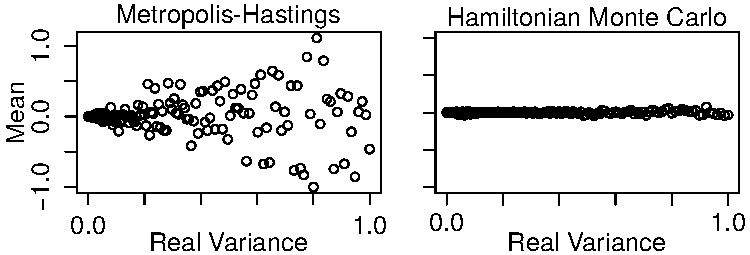
\includegraphics[width=5in]{images/MHvsHM_var.pdf}
  \caption{Sample Mean against the Real Variance of a multivariate gaussian in 150 dimensions with 1000 samples}
\end{figure}

\begin{figure}[H]
\center
  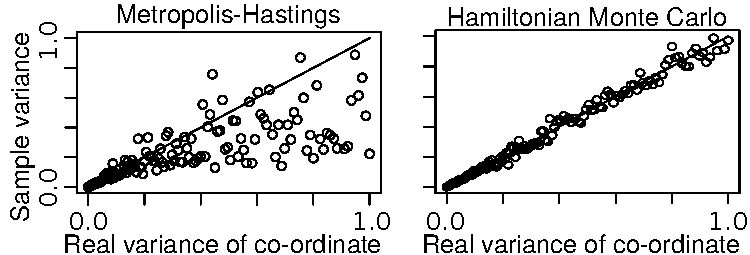
\includegraphics[width=5in]{images/MHvsHM_varcoord.pdf}
  \caption{Sample Variance against the Real Variance of a multivariate gaussian in 150 dimensions with 1000 samples}
\end{figure}
From looking at different trace and auto-correlation plots for different variables, one can clearly see much higher correlation between samples in the random walk Metropolis compared to the HMC (refer to package). Figure 2 and Figure 3 shows the sample mean and sample variance of the 1000 iterations obtained, clearly HMC outperforms MH. Further experimentation can show that even with thinning of 300 samples, HMC still outperforms MH. The results show that HMC outperforms the Metropolis Hastings in this case, this is not very surprising, as in high dimensions, intuitively it is very difficult for it to propose a point that is likely to be accepted. In fact in paper, it is shown that the computational time needed for HMC grows proportionally to $d^{5/4}$, while random walk Metropolis grows as $d^{2}$. However, tuning the parameters is not an easy task, especially in high dimensions and especially when you have no information about the shape of the target density. Below is an illustration of NUTS, as implemented in RStan, where the only information you have to provide it is the density, the differentiation and auto-tuning of all the parameters is chosen. 

\cite{rstan}
\subsection{Normal mixture models}
We compared the performance of our model to that of the Metropolis-Hastings algorithm and the NUTS method, as implemented in RStan

\begin{thebibliography}{9}

\bibitem{neal}
  Neal R.M.,
  \emph{MCMC using Hamiltonian dynamics},
  Chapter 5 of the Handbook of Markov Chain Monte Carlo,
  2012.
  
\bibitem{duane}
  Duane,S., Kennedy,A.D., Pendleton,B.J., \& Roweth,D.,
  \emph{Hybrid Monte Carlo }
  Physics Letters B, 195(2) 216-222, 1987.

\bibitem{NUTS}
  Hoffman,M.D., Gelman,A.,
  arXiv:1111.4246v1.
  
\bibitem{rstan}
  RStan, \url{http://mc-stan.org/interfaces/rstan.html}

\end{thebibliography}
\end{document}
